\documentclass[epsfig,10pt,fullpage]{article}

\newcommand{\LabNum}{6}
\newcommand{\CommonDocsPath}{../../../common/docs}
\addtolength{\textwidth}{1.5in}
\addtolength{\oddsidemargin}{-0.75in}
\addtolength{\topmargin}{-0.75in}
\addtolength{\textheight}{1.5in}
\addtolength{\evensidemargin}{0.75in}
\setlength\parindent{0pt}
\raggedbottom

\usepackage{ae,aecompl}
\usepackage{epsfig,float,times}
\usepackage[hypcap]{caption}
\usepackage[pdftex, colorlinks]{hyperref}
\usepackage{graphicx}
\usepackage[usenames, dvipsnames]{color}
\usepackage{rotating}
\usepackage{tikz}
\usetikzlibrary{automata,positioning}
\usepackage{placeins}

\widowpenalty 10000
\clubpenalty 10000

\newcommand{\red}[1]{{\color{red}\sf{#1}}}
\newcommand{\green}[1]{{\color{green}\sf{#1}}}
\newcommand{\blue}[1]{{\color{blue}\sf{#1}}}
\definecolor{PineGreen}{rgb}{0.0, 0.47, 0.44}
\definecolor{ForestGreen}{rgb}{0.13, 0.55, 0.13}
\definecolor{Brown}{rgb}{0.59, 0.29, 0.0}

\newcommand{\UPDatePublished}{Oct 2021}
\newcommand{\versnum}{21.1} %version number quartus/AMP
\newcommand{\quartusname}{Quartus\textsuperscript{\textregistered} Prime}	
\newcommand{\UPTextBar}{For \quartusname{} \versnum{}}
\newcommand{\thisyear}{2021 } %for copyright
\newcommand{\company}{FPGAcademy.org}
\newcommand{\longteamname}{FPGAcademy.org}
\newcommand{\teamname}{FPGAcademy}
\newcommand{\website}{FPGAcademy.org}

\newcommand{\productAcronym}{AMP}
\newcommand{\productNameShort}{Monitor Program}

\newcommand{\productNameMedTM}{A Monitor Program}
\newcommand{\productNameMed}{A Monitor Program}

%\newcommand{\headerLogoFilePath}[1]{#1/FPGAcademy.png}

% listings is a package that supports encapsulating source code in LaTeX conveniently
\usepackage{listings}

\def\expandparam\lstinputlisting[#1]#2{\edef\tmp{\noexpand\lstinputlisting[#1]{#2}}\tmp}

%%%%%%%%%%%%%%%%%%%% Source Code Formatting %%%%%%%%%%%%%%%%%%%%
\definecolor{globalCommentColour}{rgb}{0.588,0.588,0.588}

%%%%%%%%%%%%%%%%%%%%%%%%%%%%%%%%%%%%%%%%%%%%%%%%%%%%
% Defining language style
% NiosII ASM
\lstdefinelanguage[NiosII]{Assembler} {
  morekeywords={add, addi, and, andhi, andi, beq, bge, bgeu, bgt, bgtu, ble,  bleu, blt, bltu, bne, br, break,
  bret, call, callr, cmpeq, cmpeqi, cmpge, cmpgei, cmpgeu, cmpgeui, cmpgt, cmpgti, cmpgtu, cmpgtui, cmple,
  cmplei, cmpleu, cmpleui, cmplt, cmplti, cmpltu, cmpltui, cmpne, cmpnei, custom, div, divu, eret, flushd,
  flushda, flushi, flushp, initd, initda, initi, jmp, jmpi, ldb, ldbio, ldbu, ldbuio, ldh, ldhio, ldhu, ldhuio,
  ldw, ldwio, mov, movhi, movi, movia, movui, mul, muli, mulxss, mulxsu, mulxuu, nextpc, nop, nor, or, orhi, ori,
  rdctl, rdprs, ret, rol, roli, ror, sll, slli, sra, srai, srl, srli, stb, stbio, sth, sthio, stw, stwio,
  sub, subi, sync, trap, wrctl, wrtcl, wrprs, xor, xori, xorhi, xori},
  morekeywords=[2]{.abort, .ABORT, .align, .app-file, .ascii, .asciz, .balign, .byte, .comm, .data, .def,
  .desc, .dim, .double, .eject, .else, .end, .endef, .endif, .equ, .equiv, .err, .extern, .file, .fill, .float,
  .global, .globl, .hword, .ident, .if, .include, .int, .irp, .irpc, .lcomm, .lflags, .line, .linkonce, .ln,
  .list, .long, .macro, .mri, .nolist, .octa, .org, .p2align, .psize, .quad, .rept, .sbttl, .scl, .section,
  .set, .short, .single, .size, .sleb128, .skip, .space, .stadb, .stabn, .stabs, .string, .symver, .tag,
  .text, .title, .type, .val, .uleb128, .word},
  morekeywords=[3]{et, bt, gp, sp, fp, ea, sstatus, ra, pc, status, estatus, bstatus, ienable, ipending, cpuid,
  exception, pteaddr, tlbacc, tlbmisc, eccinj, badaddr, config, mpubase, mpuacc},
  sensitive=t,
  alsoletter=.,
  morestring=[b]",
  morecomment=[s]{/*}{*/},
  morecomment=[l]\#,
}[keywords,comments,strings]
   
%% NOTE: morekeywords=[2] are GNU directives.
   
\definecolor{niosInstructionColour}{rgb}{0.000,0.608,0.000}
\definecolor{niosDirectiveColour}{rgb}{0.000,0.000,0.902}
\definecolor{niosSpecialRegColour}{rgb}{0.000,0.000,0.000}
\definecolor{niosStringColour}{rgb}{0.808,0.482,0.000}
   
%% NOTE: To make bold use: =\bfseries\color{<colour>}
\lstdefinestyle{defaultNiosStyle} {
  language=[NiosII]{Assembler},
  stringstyle=\color{niosStringColour},
  keywordstyle=\color{niosInstructionColour},
  keywordstyle=[2]\color{niosDirectiveColour},
  keywordstyle=[3]\itshape\color{niosSpecialRegColour}
}
%%%%%%%%%%%%%%%%%%%%%%%%%%%%%%%%%%%%%%%%%%%%%%%%%%%%

%%%%%%%%%%%%%%%%%%%%%%%%%%%%%%%%%%%%%%%%%%%%%%%%%%%%
% Defining language style
% ArmA9 ASM
\lstdefinelanguage[ArmA9]{Assembler} {
  morekeywords={ADC, ADD, ADDS, AND, ANDS, B, BAL, BEQ, BGE, BGT, BL, BLT, BIC, BKPT, BLX, BNE, BX, CDP, CLZ, CMN, CMP, EOR,
  EORS, LDC, LDM, LDR, LDRB, LDRBT, LDRH, LDRSB, LDRSH, LDRT, LSL, MCR, MLA, MOV, MOVW, MOVT, MRC, MRS, MSR, MUL, MVN, ORR, PLD,
  ROR, RSB, RSC, SBC, SMLAL, SMULL, STC, STM, STR, STRB, STRBT, STRH, STRT, SUB, SUBS, SWI, SWP, SWPB, TEQ, UMLAL,
  PUSH, POP, MOVS, RORS, LSR},
  morekeywords=[2]{.abort, .ABORT, .align, .app-file, .ascii, .asciz, .balign, .byte, .comm, .data, .def,
  .desc, .dim, .double, .eject, .else, .end, .endef, .endif, .equ, .equiv, .err, .extern, .file, .fill, .float,
  .global, .globl, .hword, .ident, .if, .include, .int, .irp, .irpc, .lcomm, .lflags, .line, .linkonce, .ln,
  .list, .long, .macro, .mri, .nolist, .octa, .org, .p2align, .psize, .quad, .rept, .sbttl, .scl, .section,
  .set, .short, .single, .size, .sleb128, .skip, .space, .stadb, .stabn, .stabs, .string, .symver, .tag,
  .text, .title, .type, .val, .vectors, .uleb128, .word},
  morekeywords=[3]{SP, PC, MIDR, CTR, TCMTR, TLBTR, MPIDR, ID_PFR0, ID_PFR1, ID_DFR0, ID_MMFR0, ID_MMFR1, ID_MMFR2,
  ID_MMFR3, ID_ISAR0, ID_ISAR1, ID_ISAR2, ID_ISAR3, ID_ISAR4, CCSIDR, CLIDR, AIDR, CSSELR, TTBR0, TTRB1, TTBR2, DACR,
  DFSR, IFSR, ADFSR, AIFSR, DFAAR, IFAR, ICIALLUIS, BPIALLIS, PAR, ICIALLU, ICIMVAU, BPIALL, DCIMVAC, DCISW, V2PCWPR,
  DCCVAC, DCCSW, DDIMVAC, DCISW, TLBALLIS, TLBIMVAIS, TLBIASIDIS, TLBIMVAAIS, TLBIALL, TLBIMVA, TLBIASID, TLBIMVAA,
  PMCR, PMCNTENSET, PMCNTENCLR, PMOVSR, PMSWINC, PMSELR, PMXEVTYPER, PMXEVCNTR, PMUSERENR, PMINTENSET, PMINTENCLR,
  PRRR, NRRR, PLEIDR, PLEASR, PLEFSR, PLEUAR, PLEPCR, VBAR, MVBAR, ISR, FCSEIDR, CONTEXTIDR, TPIDRURW, TPIDRURO, TPIDRPRW},
  sensitive=f,
  alsoletter=.,
  morestring=[b]",
  morecomment=[s]{/*}{*/},
  morecomment=[l]{//},
}[keywords,comments,strings]
   
%% NOTE: morekeywords=[2] are GNU directives.
   
\definecolor{armInstructionColour}{rgb}{0.000,0.608,0.000}
\definecolor{armDirectiveColour}{rgb}{0.000,0.000,0.902}
\definecolor{armSpecialRegColour}{rgb}{0.000,0.000,0.000}
\definecolor{armStringColour}{rgb}{0.808,0.482,0.000}
   
\lstdefinestyle{defaultArmStyle} {
  language=[ArmA9]{Assembler},
  stringstyle=\color{armStringColour},
  keywordstyle=\color{armInstructionColour},
  keywordstyle=[2]\color{armDirectiveColour},
  keywordstyle=[3]\itshape\color{armSpecialRegColour}
}
%%%%%%%%%%%%%%%%%%%%%%%%%%%%%%%%%%%%%%%%%%%%%%%%%%%%

%%%%%%%%%%%%%%%%%%%%%%%%%%%%%%%%%%%%%%%%%%%%%%%%%%%%
% Defining language style
% FPGAcademy ASM
\lstdefinelanguage{ASM}{
  morekeywords = [1]{mv, mvt, mvne, mvcc, add, sub, st, ld, and, b, bne, beq, bcc, bcs},
  morekeywords = [2]{word, define},
  keywordstyle = [1]\color{ForestGreen},
  keywordstyle = [2]\color{blue},
  sensitive = true,
  morecomment = [l]{//},
}

\lstset{
  language = ASM,
  basicstyle=\small\color{black}\ttfamily,
  commentstyle=\small\color{Brown}\itshape\ttfamily,
  showstringspaces=false,
  frame=none, %lines % boxed listings
  breaklines=true,
  breakatwhitespace=true,
  tabsize=3
}
%%%%%%%%%%%%%%%%%%%%%%%%%%%%%%%%%%%%%%%%%%%%%%%%%%%%

%%%%%%%%%%%%%%%%%%%%%%%%%%%%%%%%%%%%%%%%%%%%%%%%%%%%
% Defining language style
% Java
\definecolor{javaStringColour}{rgb}{0.808,0.482,0}
%%%%%%%%%%%%%%%%%%%%%%%%%%%%%%%%%%%%%%%%%%%%%%%%%%%%

%%%%%%%%%%%%%%%%%%%%%%%%%%%%%%%%%%%%%%%%%%%%%%%%%%%%
% Defining language style
% C
\definecolor{CStringColour}{rgb}{0.808,0.482,0}

\lstset{
  language = C,
  basicstyle=\small\color{black}\ttfamily, 
  commentstyle=\small\color{PineGreen}\itshape\ttfamily,
  keywordstyle=\small\color{blue}\bfseries\ttfamily,
  showstringspaces=false,
  frame=none, %lines % boxed listings
  breaklines=true,
  breakatwhitespace=true,
  tabsize=3
}
%%%%%%%%%%%%%%%%%%%%%%%%%%%%%%%%%%%%%%%%%%%%%%%%%%%%

%%%%%%%%%%%%%%%%%%%%%%%%%%%%%%%%%%%%%%%%%%%%%%%%%%%%
% Defining language style
% Verilog
\definecolor{verilogCommentColour}{rgb}{0.000,0.502,0.000}

\lstdefinestyle{defaultVerilogStyle} {
  language={Verilog},
  keywordstyle=\color{blue},
  commentstyle=\color{verilogCommentColour}
}
%%%%%%%%%%%%%%%%%%%%%%%%%%%%%%%%%%%%%%%%%%%%%%%%%%%%

%%%%%%%%%%%%%%%%%%%%%%%%%%%%%%%%%%%%%%%%%%%%%%%%%%%%
% Defining language style
% VHDL
\lstdefinestyle{defaultVHDLStyle} {
  language={VHDL},
  keywordstyle=\color{blue},
  commentstyle=\color{verilogCommentColour}
}
%%%%%%%%%%%%%%%%%%%%%%%%%%%%%%%%%%%%%%%%%%%%%%%%%%%%

%%%%%%%%%%%%%%%%%%%%%%%%%%%%%%%%%%%%%%%%%%%%%%%%%%%%
% Defining language style
% LaTeX
\lstdefinelanguage[LocalLaTeX]{TeX}[LaTeX]{TeX}{moretexcs={bf, it, sf, lstset},}

\lstdefinestyle{defaultLocalLatexStyle} {
  language=[LocalLatex]{TeX},
  keywordstyle=\color{blue}\bfseries,
  keywordstyle=[2]\color{blue},
  keywordstyle=[3]\color{blue}\bfseries
}
%%%%%%%%%%%%%%%%%%%%%%%%%%%%%%%%%%%%%%%%%%%%%%%%%%%%

%%%%%%%%%%%%%%%%%%%%%%%%%%%%%%%%%%%%%%%%%%%%%%%%%%%%
% Defining language style
% Default
\lstset{
  basicstyle=\small\color{black}\ttfamily,
  commentstyle=\small\color{globalCommentColour}\itshape\ttfamily,
  keywordstyle=\small\color{blue}\bfseries\ttfamily,
  showstringspaces=false,
  frame=none, %lines % boxed listings
  breaklines=true,
  breakatwhitespace=true,
  tabsize=3
}
%%%%%%%%%%%%%%%%%%%%%%%%%%%%%%%%%%%%%%%%%%%%%%%%%%%%


\hypersetup{
  pdftitle={Digital Logic Lab Exercise \LabNum},
  linkcolor=blue,
  hyperindex=true,
  pdfauthor={FPGAcademy.org},
  pdfkeywords={FPGAcademy.org, FPGAcademy, Lab, Exercise, Digital Logic},
  bookmarks,
  bookmarksopen=false,
  filecolor=blue,
  pdfstartview={FitH},
  urlcolor=blue,
  plainpages=false,
  pdfpagelabels=true,
  linkbordercolor={1 1 1} %no color for link border
}



\begin{document}

\centerline{\huge Digital Logic}
~\\
\centerline{\huge Laboratory Exercise \LabNum}
~\\
\centerline{\large Adders, Subtractors, and Multipliers}
~\\

The purpose of this exercise is to examine arithmetic circuits that add, subtract,
and multiply numbers. Each circuit will be described in VHDL and implemented on an 
Intel\textsuperscript{\textregistered} FPGA DE10-Lite, DE0-CV, DE1-SoC, or DE2-115 board.

\section*{Part I}
\addcontentsline{toc}{1}{Part I}
Consider again the four-bit ripple-carry adder circuit used in lab exercise 2; its diagram is reproduced in Figure~\ref{fig:ripple_carry}.

\begin{figure}[H]
\centerline{
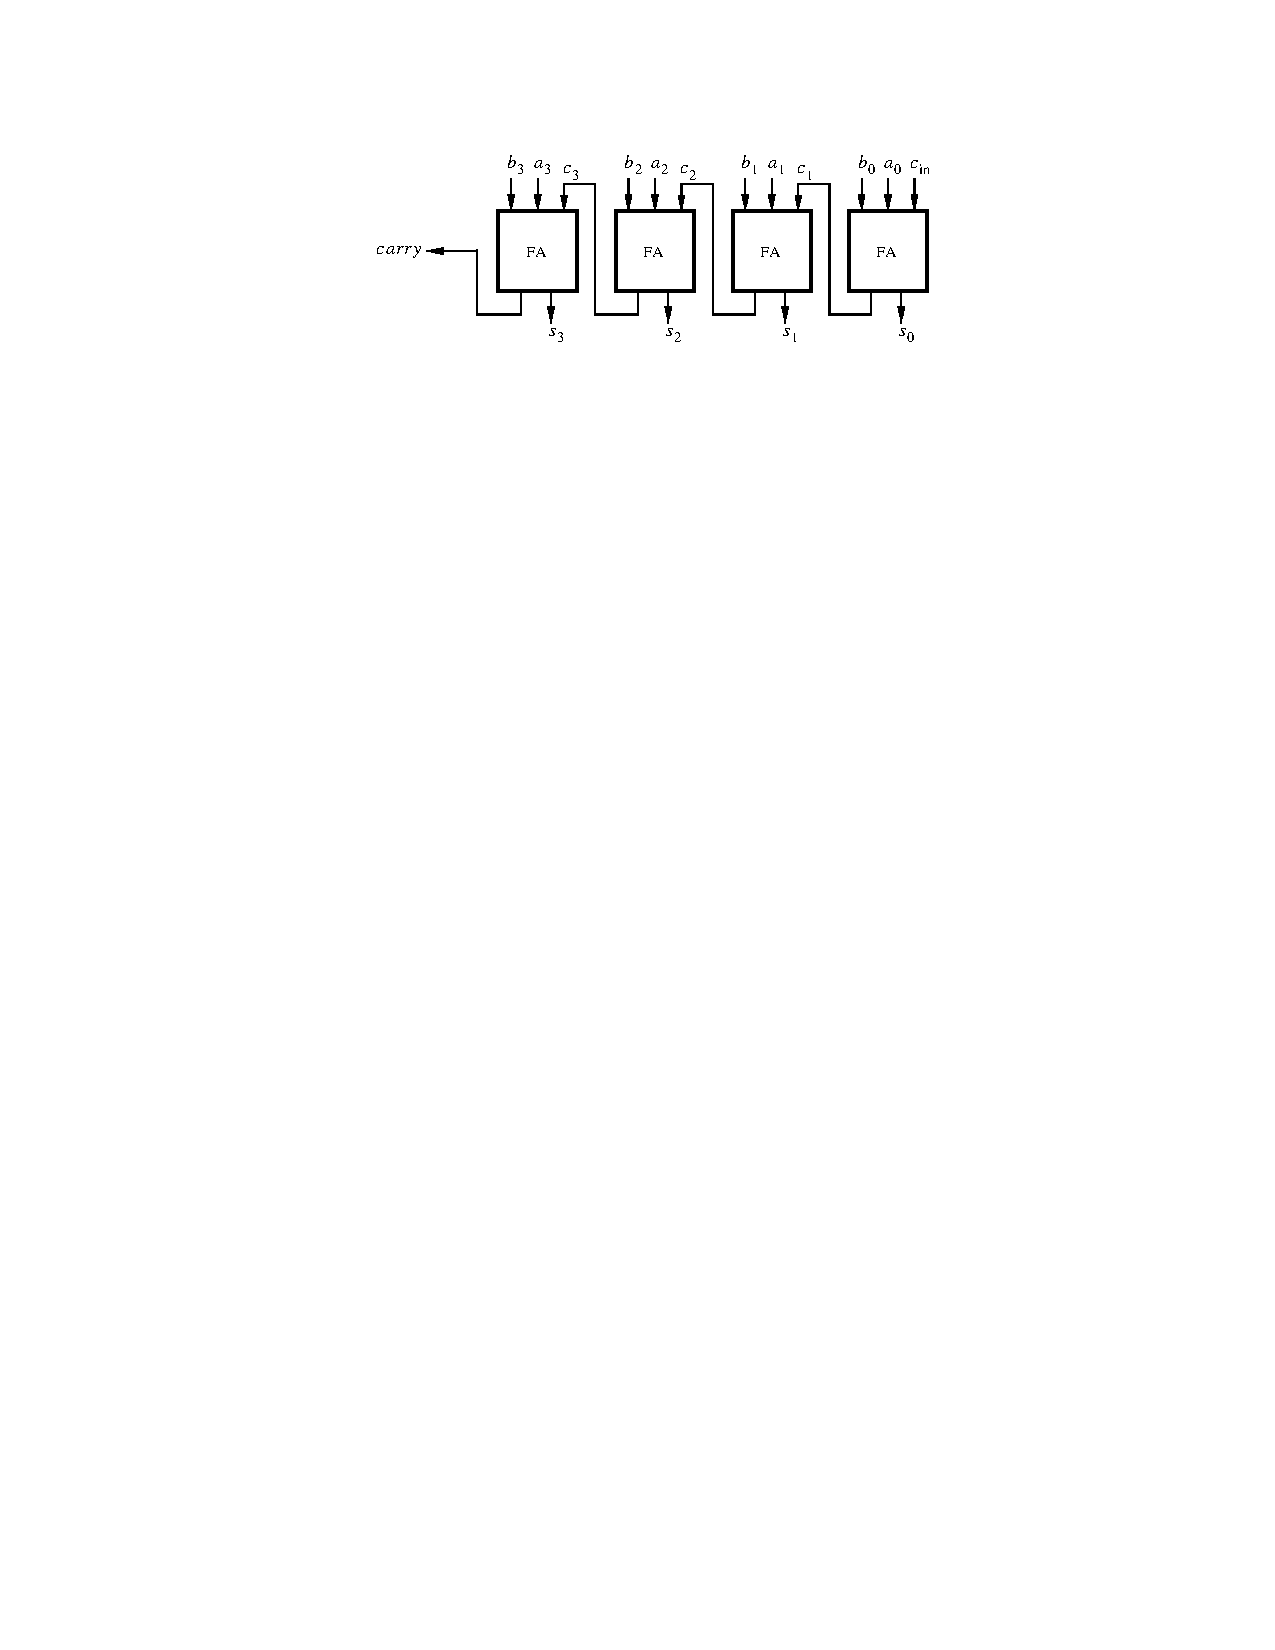
\includegraphics{figures/ripple_carry}}
\caption{A four-bit ripple carry adder.}
\label{fig:ripple_carry}
\end{figure}

This circuit can be implemented using a '+' sign in VHDL. For example, the following code fragment adds {\it n}-bit numbers $A$ and $B$ to produce outputs $sum$ and $carry$:

\begin{center}
\begin{minipage}[t]{12.5 cm}
\begin{tabbing}
ZZ\=ZZ\=ZZ\=ZZ\=ZZ\=ZZ\=ZZ\=ZZ\=ZZ\=ZZ\=ZZ\kill
\>LIBRARY ieee;\\
\>USE ieee.std\_logic\_1164.all;\\
\>USE ieee.std\_logic\_arith.all;\\
\>USE ieee.std\_logic\_signed.all;\\
\>\ldots \\
\>SIGNAL sum : STD\_LOGIC\_VECTOR(n-1 DOWNTO 0);\\
\>\ldots \\
\>sum $<$= A + B;\\
\end{tabbing}
\end{minipage}
\end{center}

Use this construct to implement a circuit shown in Figure~\ref{fig:accumulator}. This
circuit, which is often called an {\it accumulator}, is used to add the value of an input
$A$ to itself repeatedly. The circuit includes a carry out from the adder, as well as an
{\it overflow} output signal. If the input $A$ is considered as a 2's-complement number, 
then {\it overflow} should be set to~1
in the case where the output {\it sum} produced does not represent a correct
2's-complement result.

~\\
Perform the following steps:
\begin{enumerate}
\item Create a new Quartus\textsuperscript{\textregistered} project. Write VHDL code that describes the 
circuit in Figure~\ref{fig:accumulator}.
\item Connect input $A$ to switches {\it SW}$_{7-0}$, use {\it KEY}$_0$ as an 
active-low asynchronous reset, and use {\it KEY}$_1$ as a manual clock input. The sum 
from the adder should be displayed on the red lights {\it LEDR}$_{7-0}$, the registered 
carry signal should be displayed on {\it LEDR}$_{8}$, and the registered {\it overflow} 
signal should be displayed on {\it LEDR}$_{9}$. Show the registered values of {\it A}
and {\it S} as hexadecimal numbers on the 7-segment displays HEX$3-2$ and HEX$1-0$. 
\item Make the necessary pin assignments needed to implement the circuit on your
DE-series board, and compile the circuit.
\item Use timing simulation to verify the correct operation of the
circuit. Once the simulation works properly, generate a .qsf file in Quartus, upload it to the NO-IDE lab of LabsLand, 
and test it by using different values of~$A$. Be sure to check that the {\it overflow} 
output works correctly.
\item For more info, if you have a FPGA chip, you can download the compiled circuit into the FPGA chip.
\end{enumerate}

\begin{figure}[H]
\centerline{
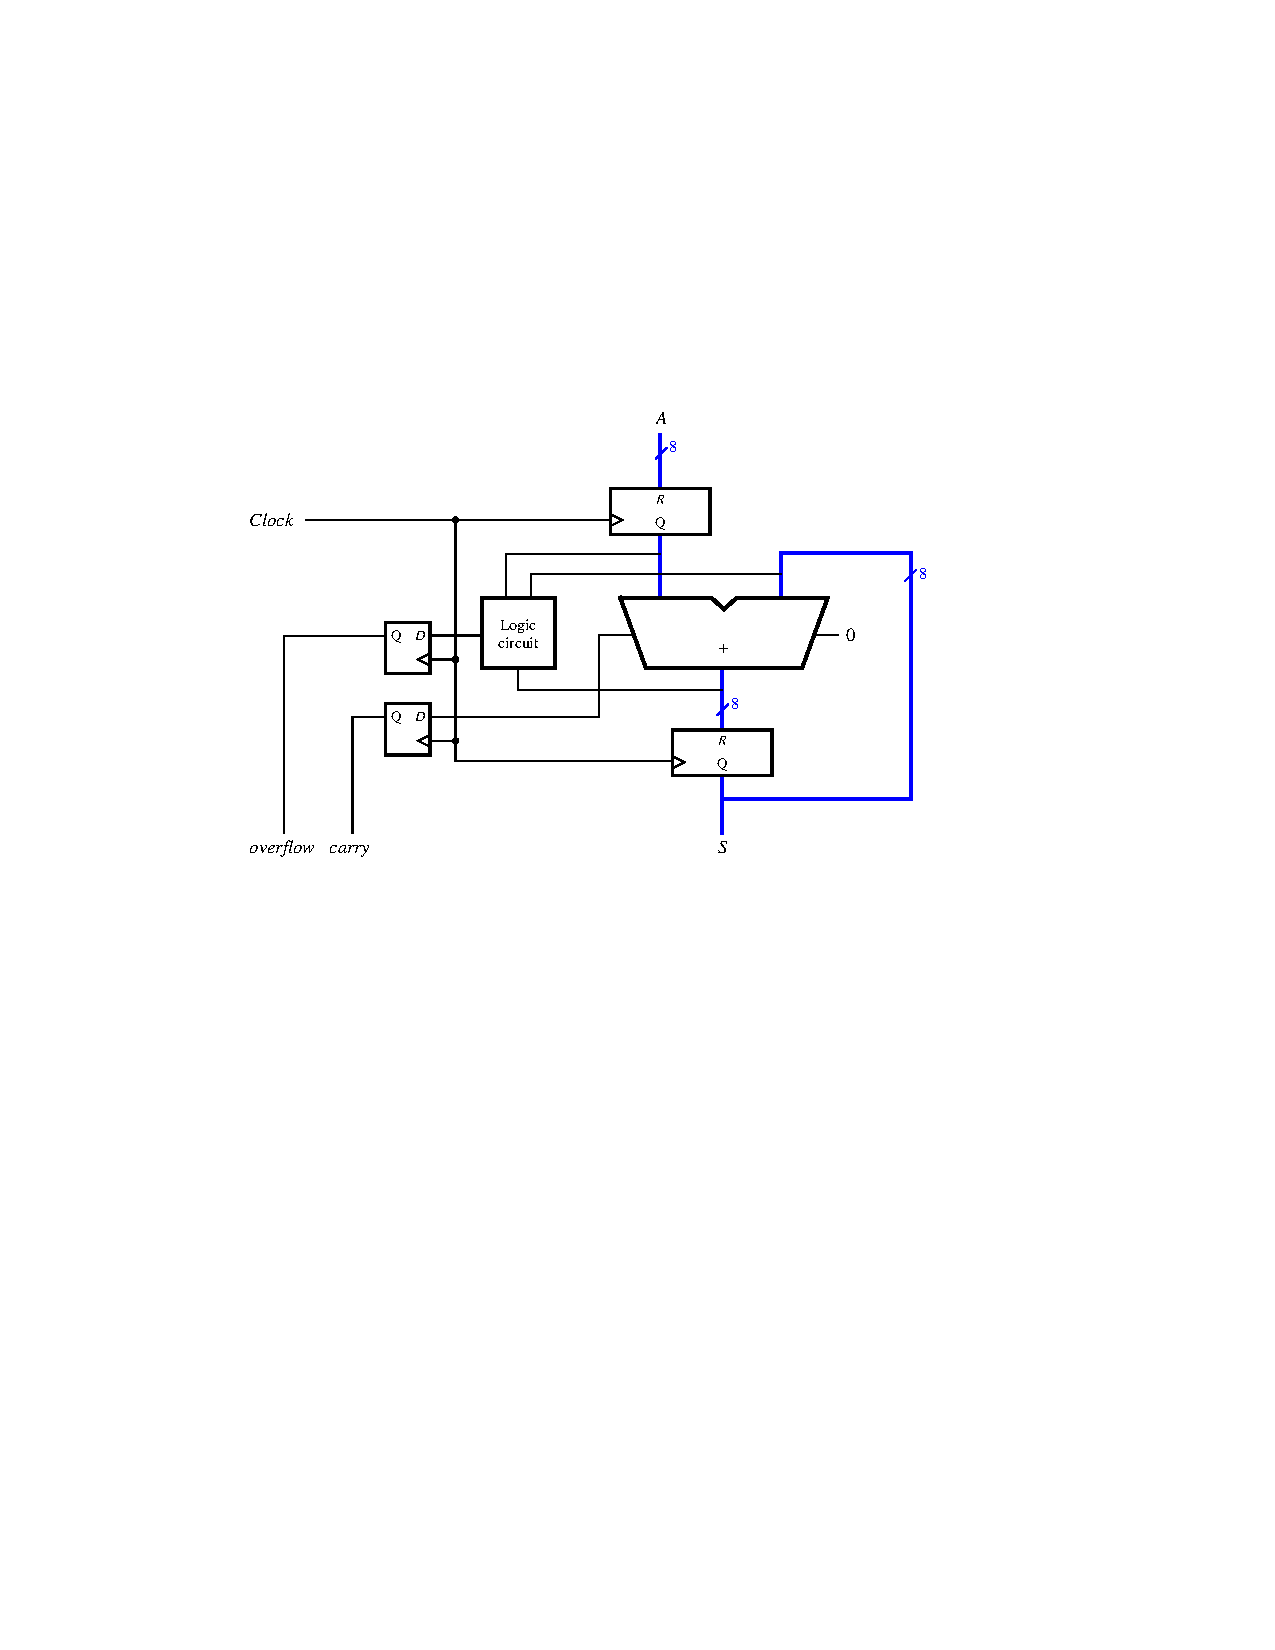
\includegraphics{figures/accumulator}}
\caption{An eight-bit accumulator circuit.}
\label{fig:accumulator}
\end{figure}

\section*{Part II}
\addcontentsline{toc}{2}{Part II}
Extend the circuit from Part I to be able to both add and subtract numbers. To do so,
introduce an {\it add\_sub} input to your circuit. When {\it add\_sub} is 1, your circuit should
subtract $A$ from $S$, and when {\it add\_sub} is 0 your circuit should add 
$A$ to $S$ as in Part I.

\section*{Part III}
\addcontentsline{toc}{3}{Part III}
Figure~\ref{fig:binary_multiplication}$a$ gives an example of paper-and-pencil multiplication $P = A \times B$, where $A = 11$ and $B = 12$.

\begin{figure}[H]
	\begin{center}
		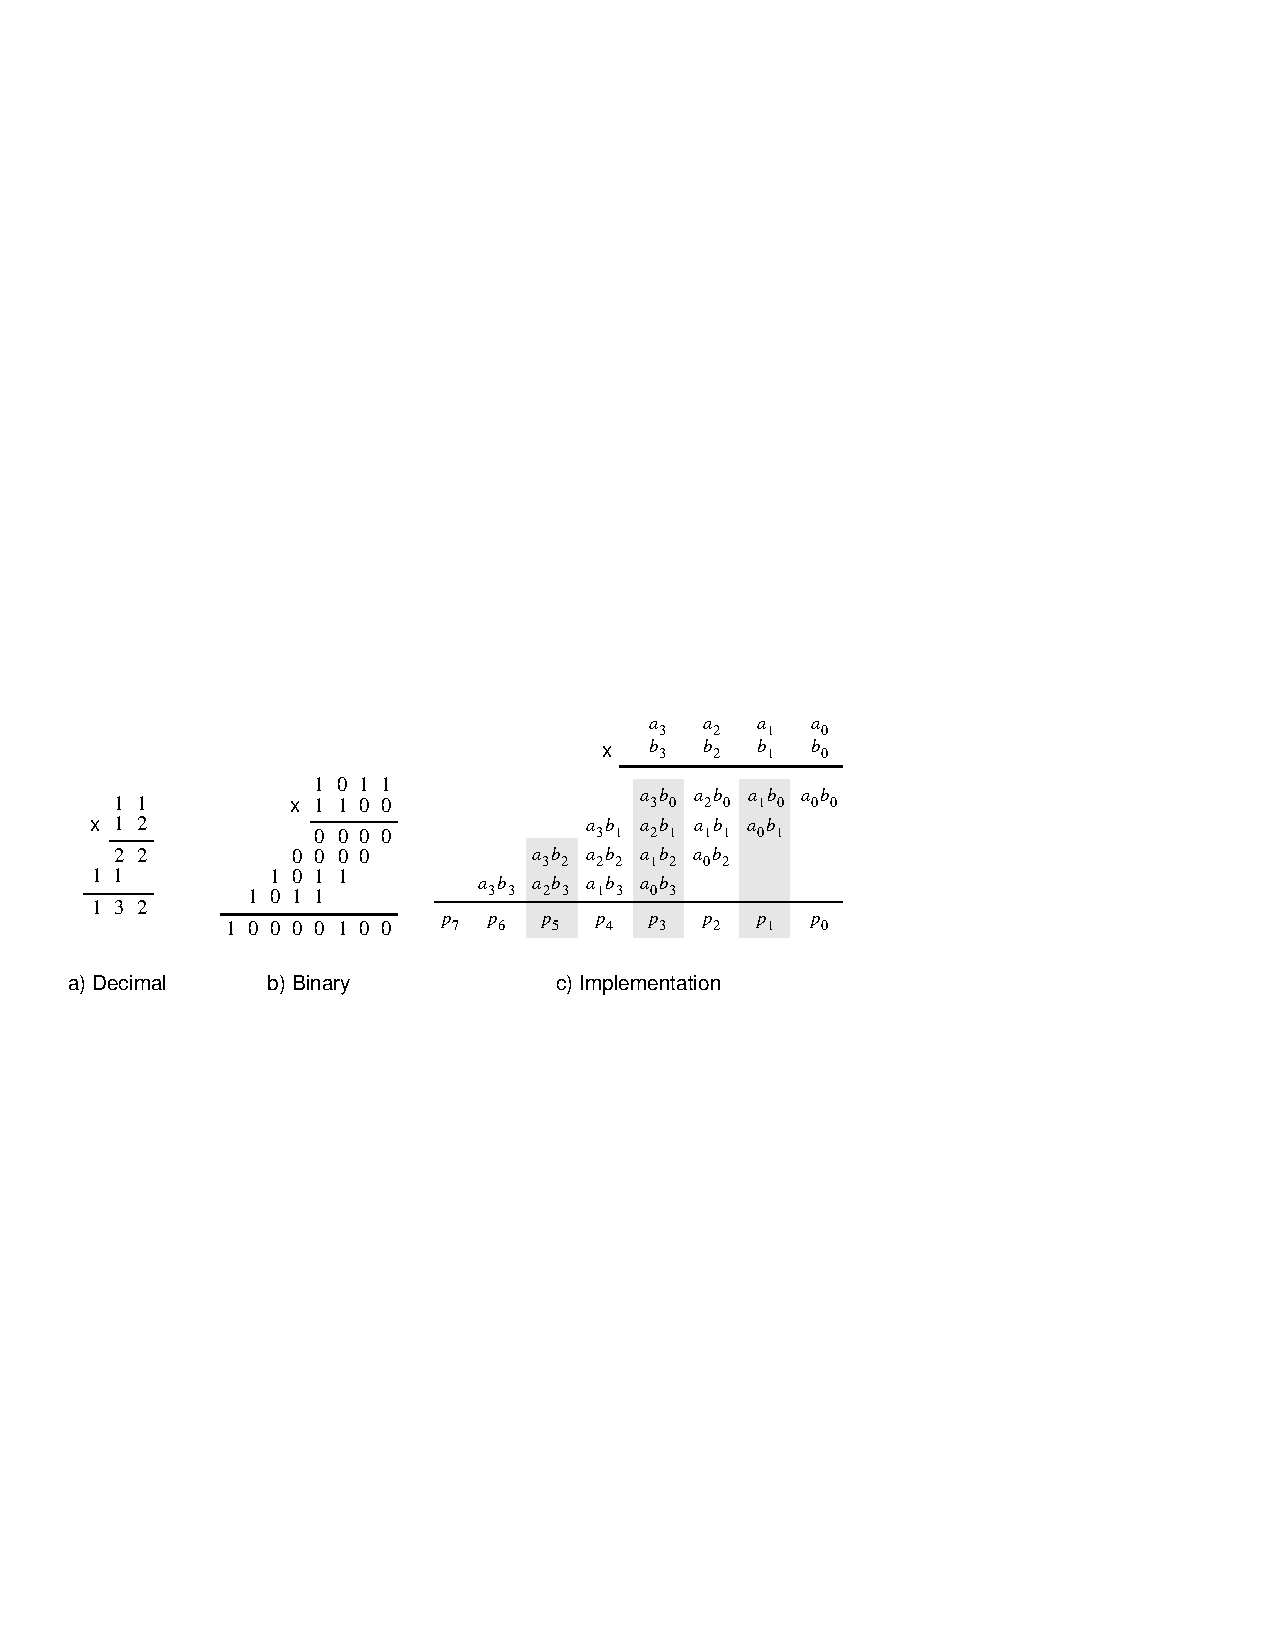
\includegraphics{figures/figure3.pdf}
	\end{center}
	\caption{Multiplication of binary numbers.}
	\label{fig:binary_multiplication}
\end{figure}

We compute $P = A \times B$ as an addition of summands. The first summand is equal to $A$ times the ones digit of $B$.
The second summand is $A$ times the tens digit of $B$, shifted one position to the left. We add the two summands to form the product $P = 132$.

~\\
Part $b$ of the figure shows the same example using four-bit binary numbers.
To compute $P = A \times B$, we first form summands by multiplying $A$ by each digit of $B$. Since each digit of
$B$ is either 1 or 0, the summands are either shifted versions of $A$ or 0000. Figure ~\ref{fig:binary_multiplication}$c$
shows how each summand can be formed by using the Boolean AND operation of $A$ with the appropriate bit of $B$.

~\\
A four-bit circuit that implements $P = A \times B$ is illustrated in Figure~\ref{fig:array_mult}. Because of its
regular structure, this type of multiplier circuit is called an {\it array multiplier}. The shaded areas correspond to the shaded columns in Figure~\ref{fig:binary_multiplication}$c$. In each row of the multiplier AND gates are used to produce the summands,
and full adder modules are used to generate the required sums.

\begin{figure}[htb]
	\begin{center}
		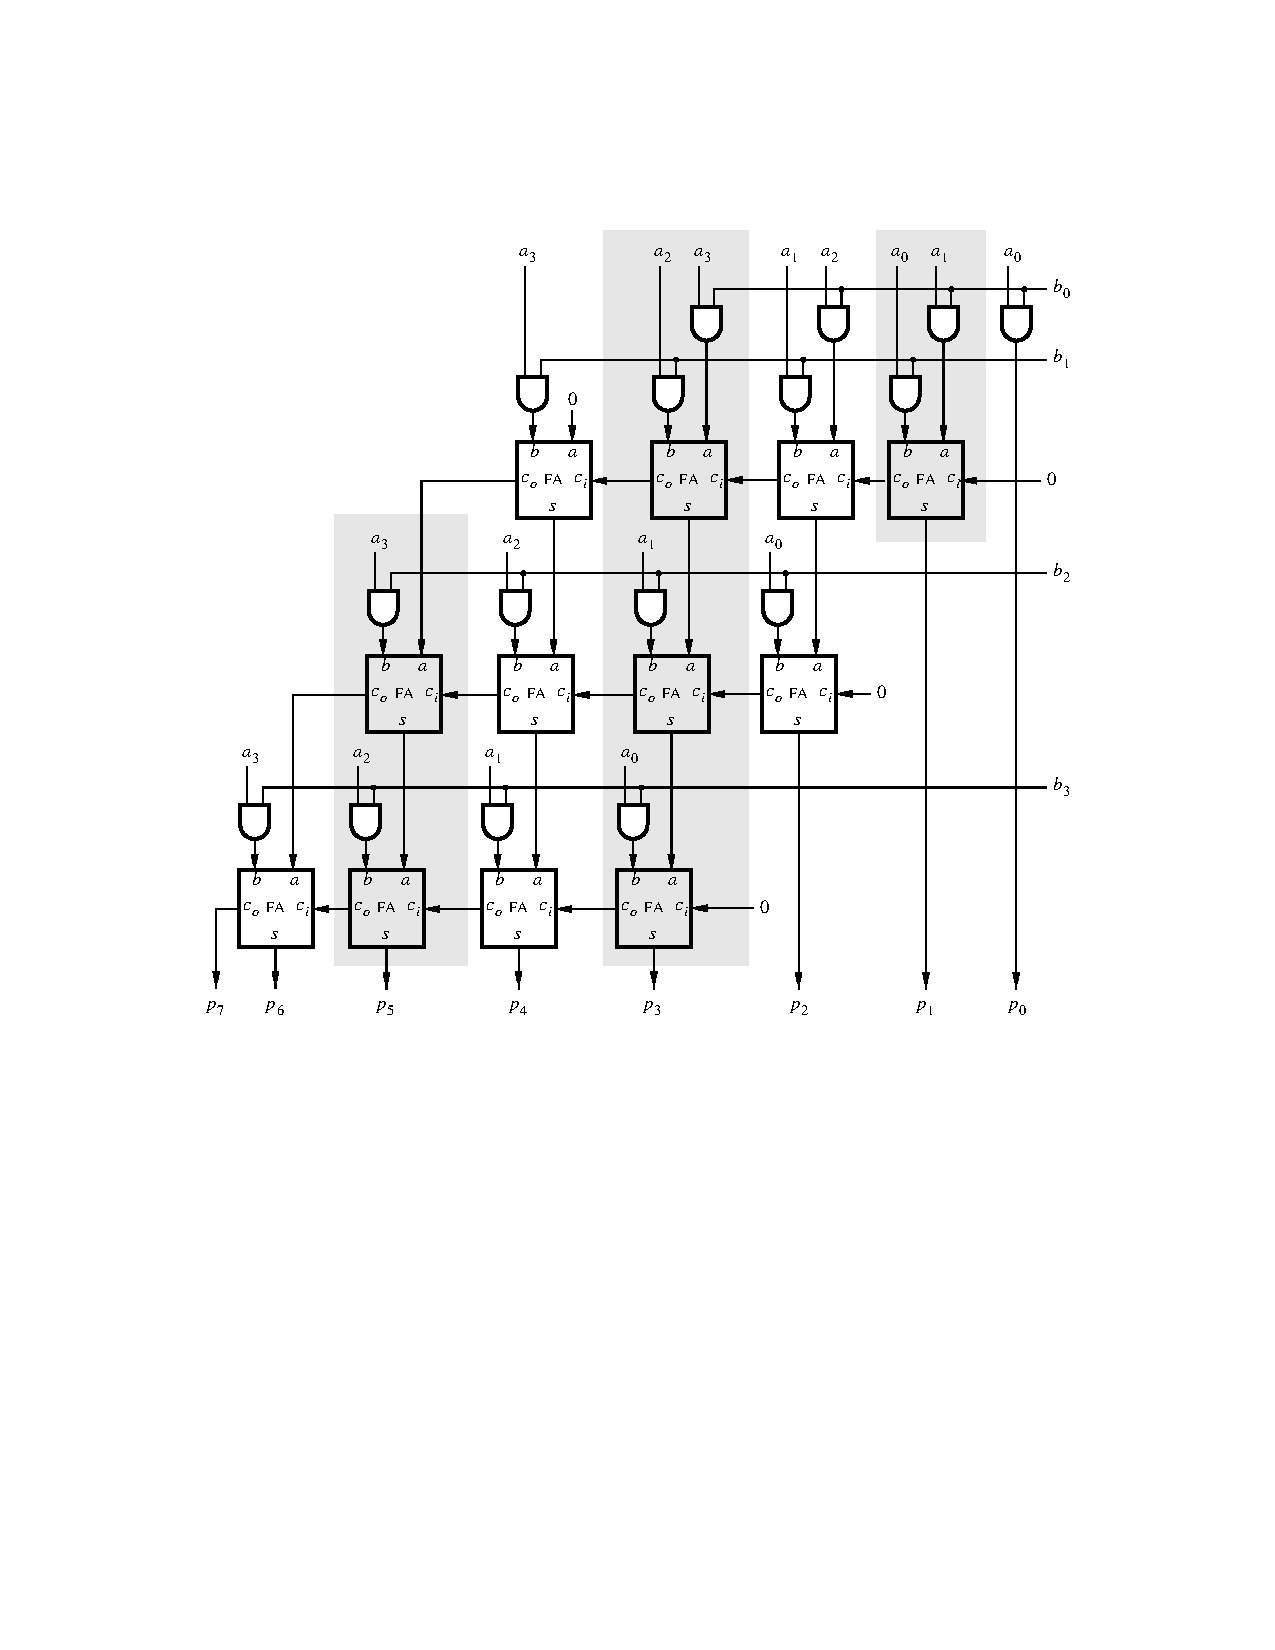
\includegraphics[]{figures/figure4.pdf}
	\end{center}
	\caption{An array multiplier circuit.}
	\label{fig:array_mult}
\end{figure}

Perform the following steps to implement the array multiplier circuit:

\begin{enumerate}
\item Create a new Quartus project.
\item Generate the required VHDL file. Use switches {\it SW}$_{7-4}$ to represent the 
number $A$ and switches {\it SW}$_{3-0}$ to represent $B$. The hexadecimal values of~$A$ 
and $B$ are to be displayed on the 7-segment displays {\it HEX}2 and {\it HEX}0, respectively.
The result ~$P = A \times B$~ is to be displayed on {\it HEX}$5-4$.
\item Make the necessary pin assignments needed to implement the circuit on your
DE-series board, and compile the circuit.
\item Use simulation to verify your design.
\item Generate a .qsf file in Quartus, upload it to the NO-IDE lab of LabsLand and test its functionality.
\item For more info, if you have a FPGA chip, you can download the compiled circuit into the FPGA chip.
\end{enumerate}

\section*{Part IV}
\addcontentsline{toc}{4}{Part IV}
In Part III, an array multiplier was implemented using full adder modules. At a higher level, a row of full adders functions as an $n$-bit adder and the array multiplier circuit can be represented as shown in Figure~\ref{fig:array_mult_adders}.

\begin{figure}[H]
\centerline{
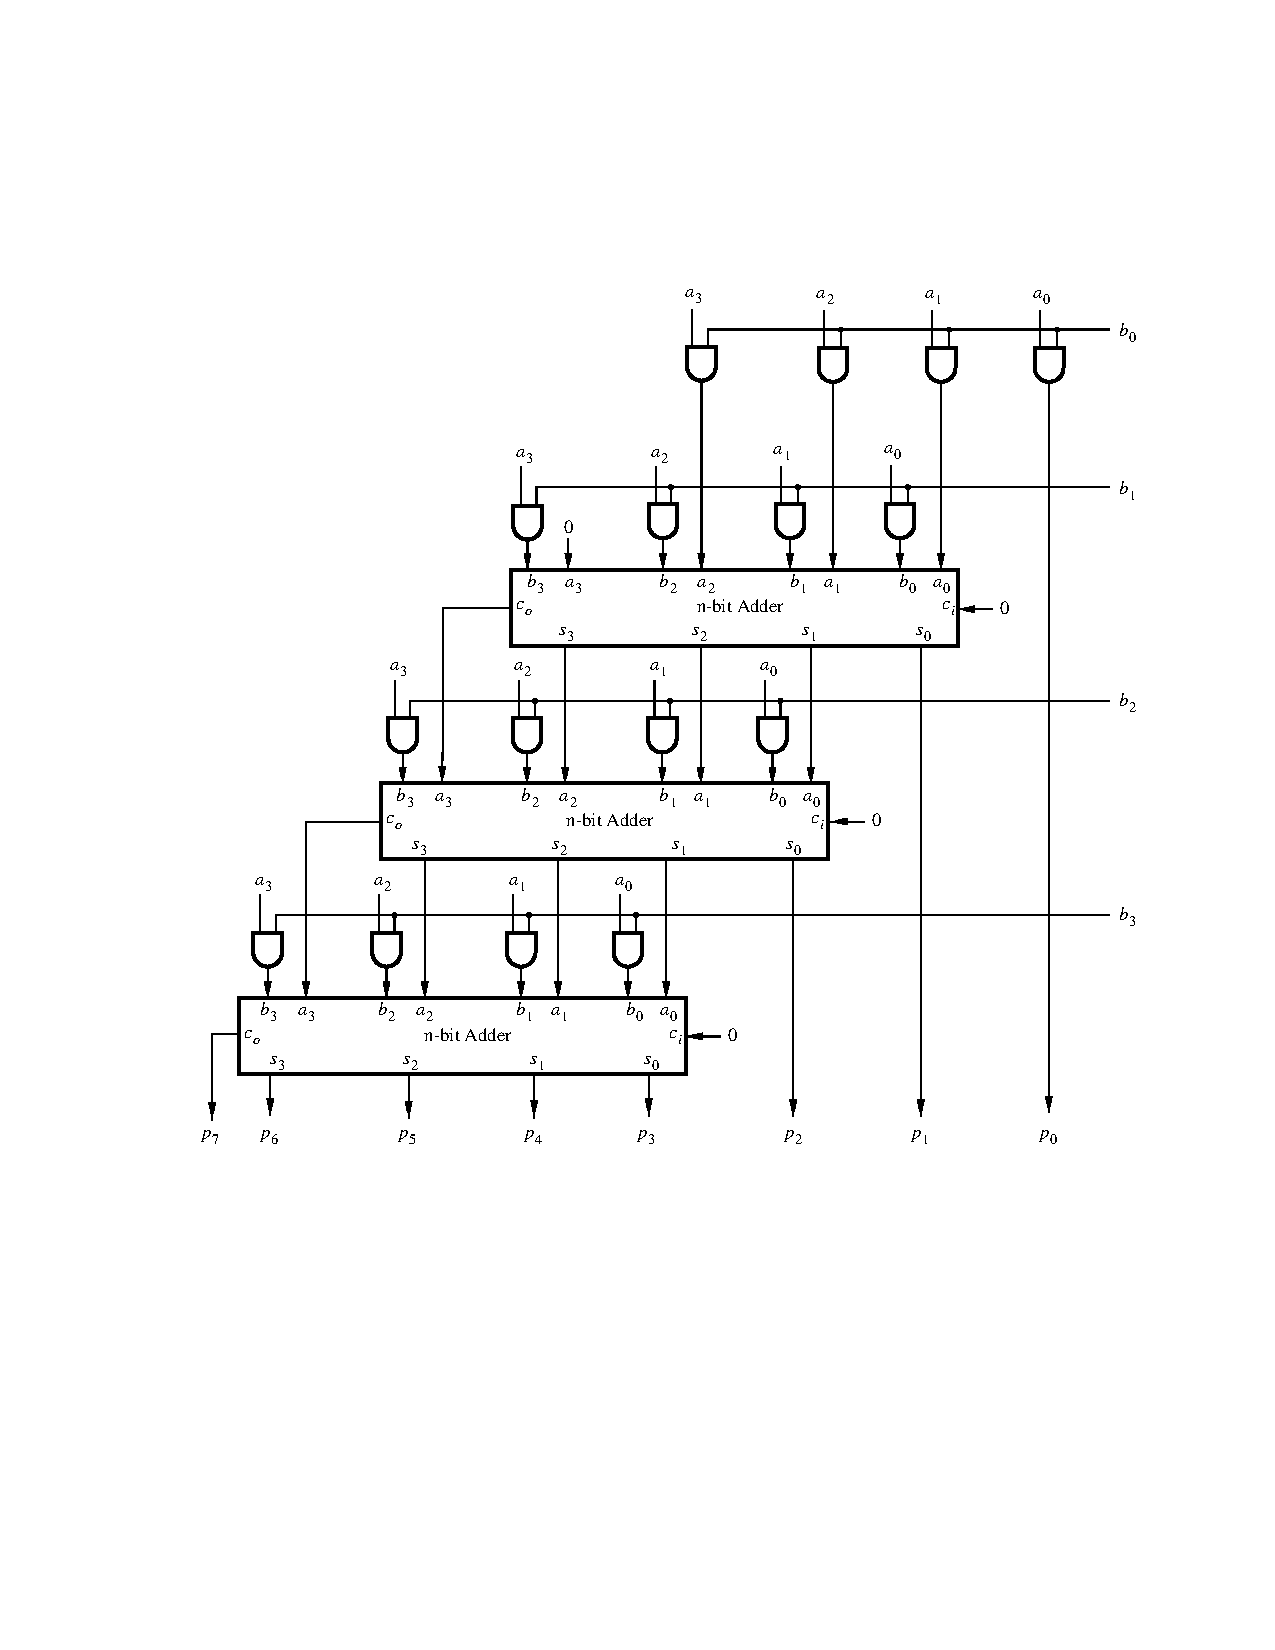
\includegraphics{figures/array_mult_adders}}
\caption{An array multiplier implemented using $n$-bit adders.}
\label{fig:array_mult_adders}
\end{figure}

Each $n$-bit adder adds a shifted version of $A$ for a given row and the {\it partial
product} of the row above. Abstracting the multiplier circuit as a sequence of additions 
allows us to build larger multipliers. The multiplier should consist of n-bit adders
arranged in a structure shown in Figure~\ref{fig:array_mult_adders}. Use this approach to 
implement an 8 {\sf x} 8 multiplier circuit with registered
inputs and outputs, as shown in Figure~\ref{fig:registered_mult}.

\begin{figure}[H]
\centerline{
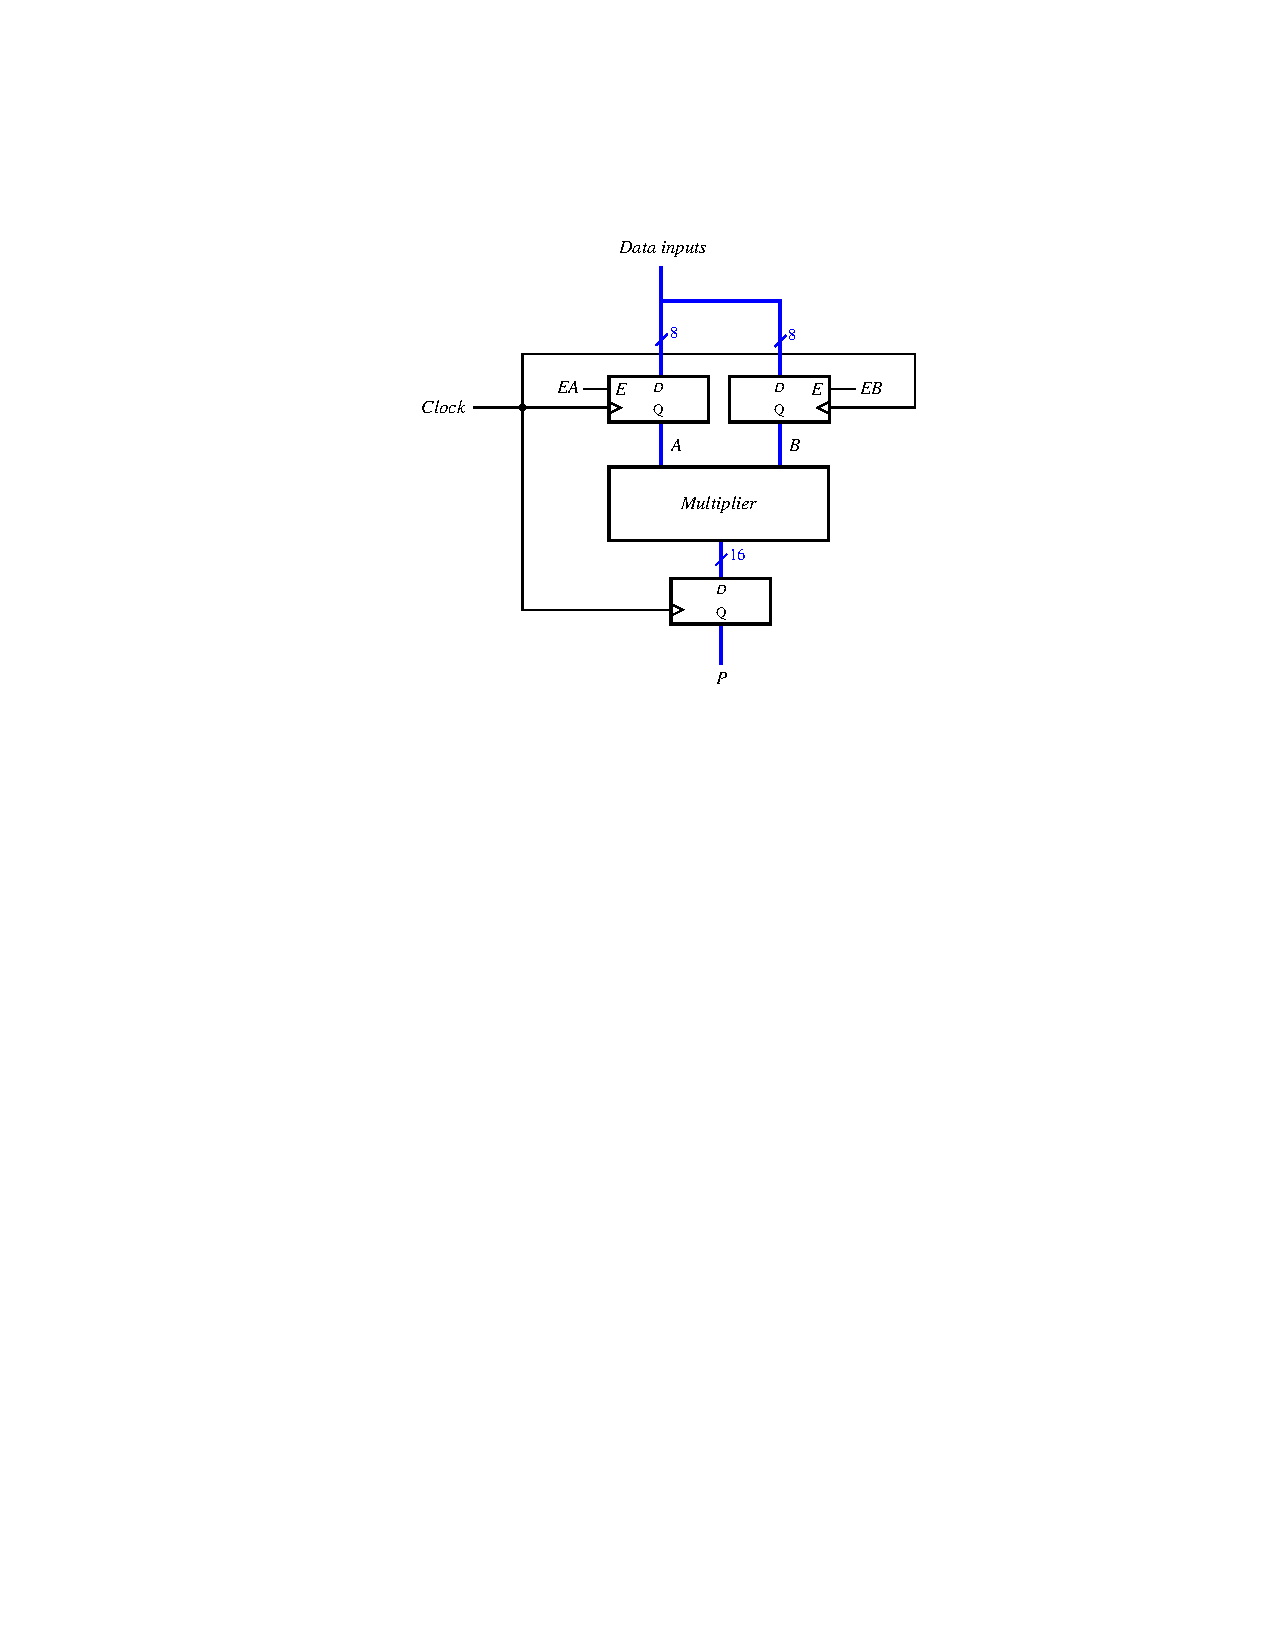
\includegraphics{figures/registered_mult}}
\caption{A registered multiplier circuit.}
\label{fig:registered_mult}
\end{figure}

Perform the following steps:
\begin{enumerate}
\item Create a new Quartus project and write the required VHDL file.
\item Use switches {\it SW}$_{7-0}$ to provide the data inputs to the circuit. Use
{\it SW}$_9$ as the enable signal {\it EA} for register {\it A}, and use {\it SW}$_8$
as the enable for register {\it B}.  When {\it SW}$_9 = 1$ display the contents of
register A on the red lights LEDR, and display the contents of register B on these lights
when {\it SW}$_8 = 1$. Use {\it KEY}$_0$ as a synchronous reset input, and use 
{\it KEY}$_1$ as a manual clock signal.  Show the product~$P = A \times B$~ as a
hexadecimal number on the 7-segment displays {\it HEX3-0}.
\item Make the necessary pin assignments needed to implement the circuit on your
DE-series board, and compile the circuit.
\item Generate a .qsf file in Quartus, upload it to the NO-IDE lab of LabsLand and test the functionality of your design by inputting various data values and observing
the generated products.
\item For more info, if you have a FPGA chip, you can download the compiled circuit into the FPGA chip.
\end{enumerate}

\section*{Part V}
\addcontentsline{toc}{5}{Part V}
Part IV showed how to implement multiplication $A \times B$ as a sequence of additions, 
by accumulating the shifted versions of $A$ one row at a time. Another way to implement 
this circuit is to perform addition using an adder tree.

An adder tree is a method of adding several numbers together in a parallel fashion. This 
idea is illustrated in Figure~\ref{fig:adder_tree}. In the figure, numbers 
$A$, $B$, $C$, $D$, $E$, $F$, $G$, and $H$ are added together in parallel.
The addition $A + B$ happens simultaneously with $C + D$, $E + F$ and $G + H$. The 
result of these operations are then added in parallel
again, until the final sum $P$ is computed.

\begin{figure}[H]
\centerline{
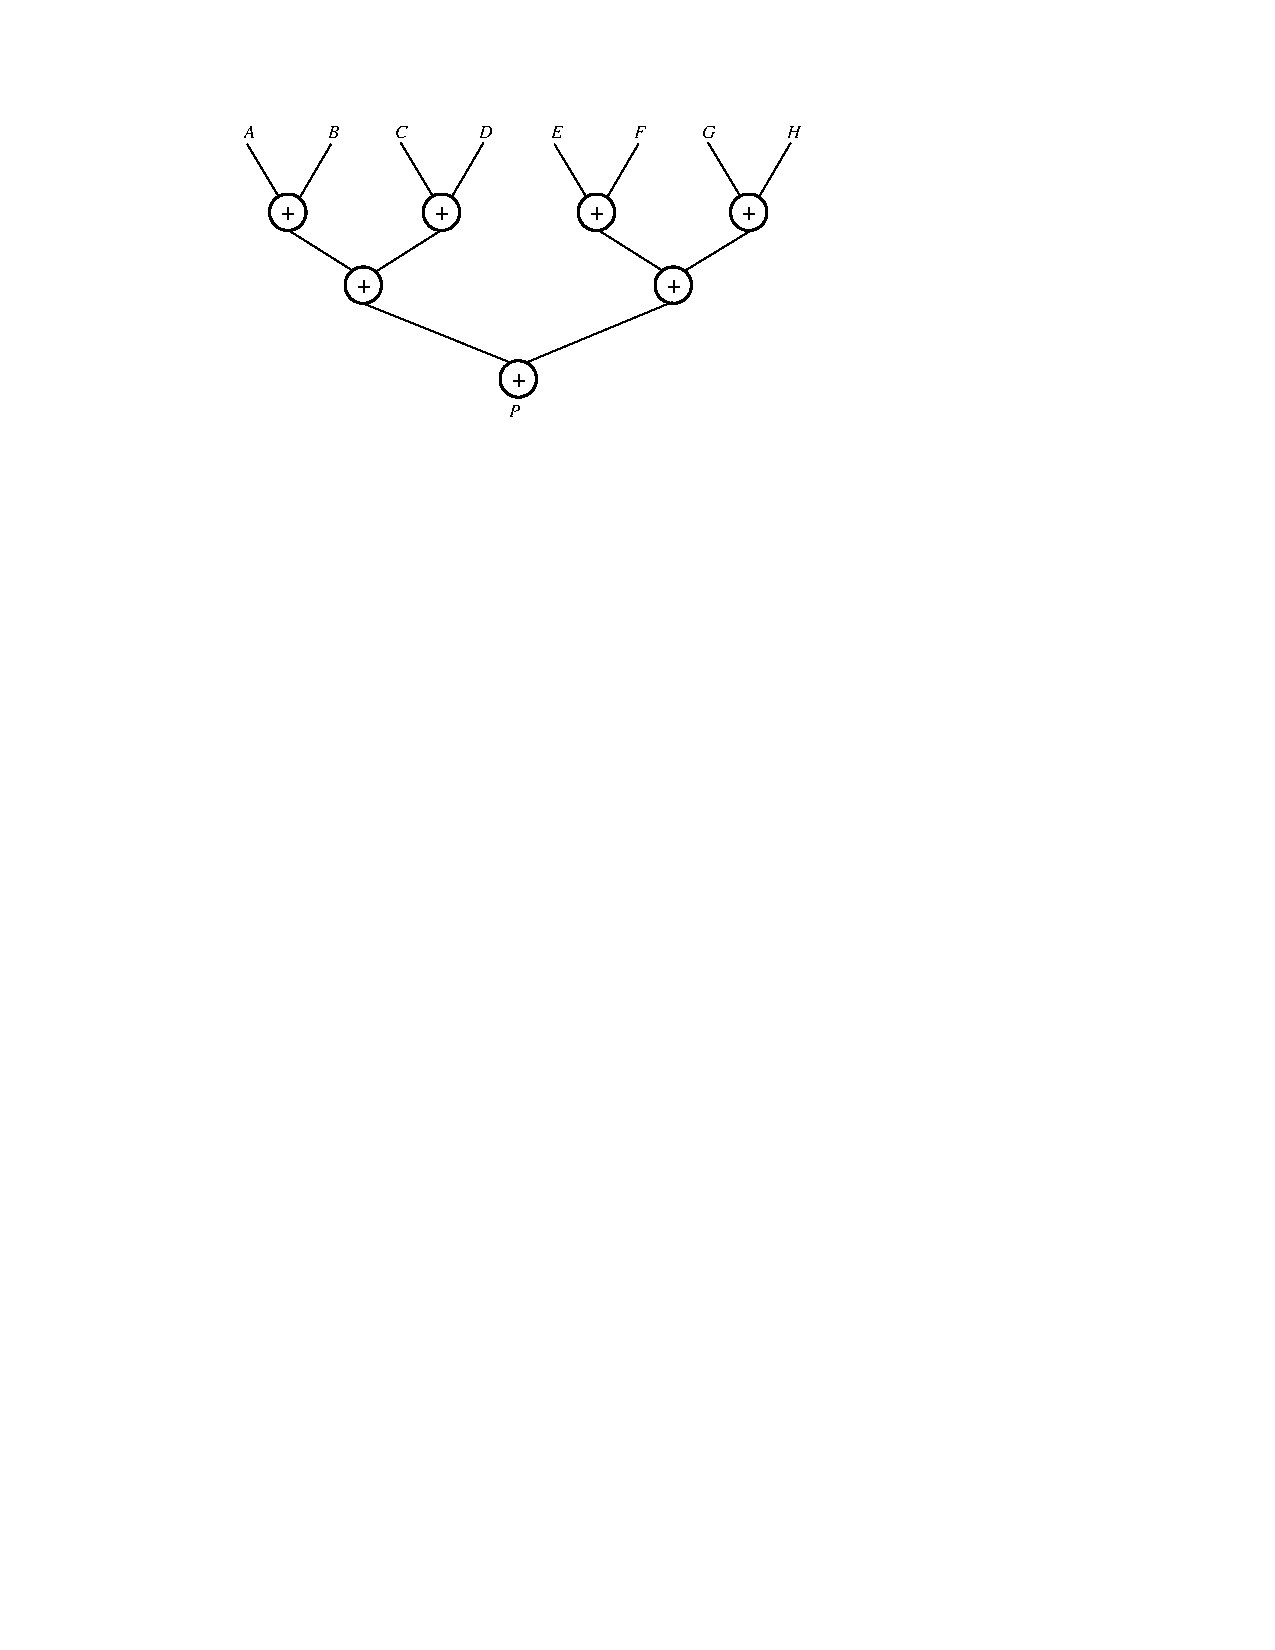
\includegraphics{figures/adder_tree}}
\caption{An example of adding 8 numbers using an adder tree.}
\label{fig:adder_tree}
\end{figure}

In this part you are to implement an 8 {\sf x} 8 multiplier circuit by using the adder-tree
approach. Inputs $A$ and $B$, as well as the output $P$ should be registered as in Part IV. 


%%%%%%%%%%%%%%%%%%%%%%%%%%%%%%%%%%%%%%%%
%%% FPGAcademy Copyright Information %%%
%%%%%%%%%%%%%%%%%%%%%%%%%%%%%%%%%%%%%%%%

%Always put the copyright on a new page (clear page), with some vertical space from top
\clearpage
\vspace{1in}

\noindent

Copyright {\copyright} FPGAcademy.org. All rights reserved. FPGAcademy and the 
FPGAcademy logo are trademarks of FPGAcademy.org.  This document is provided 
"as is", without warranty of any kind, express or implied, including but not 
limited to the warranties of merchantability, fitness for a particular purpose 
and noninfringement. In no event shall the authors or copyright holders be 
liable for any claim, damages or other liability, whether in an action of 
contract, tort or otherwise, arising from, out of or in connection with the 
document or the use or other dealings in the document.
~\\
~\\
**Other names and brands may be claimed as the property of others.


\end{document}
